\documentclass{article}
\usepackage[UTF8]{ctex}
\usepackage{graphicx}		%插入图片
\usepackage{indentfirst}	%首行缩进
\usepackage{float}			%浮动体
\usepackage{amsmath}		%矩阵

\setlength{\parindent}{2em}	%首行缩进2汉字

\usepackage{graphicx} %插入图片的宏包
\usepackage{float} %设置图片浮动位置的宏包
\usepackage{subfigure} %插入多图时用子图显示的宏包

\begin{document}

\title{第12组数据探索}
\maketitle						%生成标题
\section{数据阐述}

到现在为止,我们收集了包含YouTube频道的id和名字、Social Blade的排名和评分、上传视频数量、订阅量、视频总播放量、视频种类、创建时间、按订阅量的排名、按总播放量的排名、在所在国家的排名、在同类型频道中的排名、最近30天的订阅者数量、最近30天的视频播放量、最高和最低的月收入年收入估计、频道所在国家及这些国家的失业率、人口总数、人均GDP。未来可能会根据想要探究的问题收集更多数据。

\section{数据分析}

我们首先分析了订阅人数、总播放量、近30天播放量与类型的关系,如下图所示。
\begin{figure}[H] %H为当前位置,!htb为忽略美学标准,htbp为浮动图形
\centering %图片居中
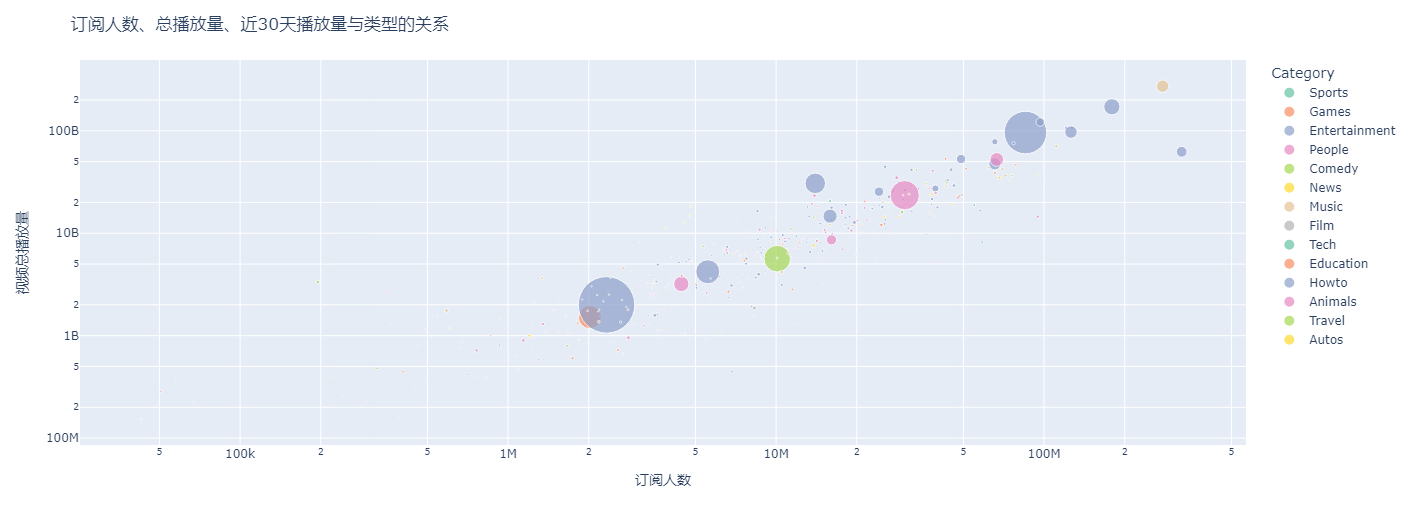
\includegraphics[width=0.7\textwidth]{pic/p1} %插入图片,[]中设置图片大小,{}中是图片文件名
%\caption{Main name 2} %最终文档中希望显示的图片标题
\label{Fig.p1} %用于文内引用的标签
\end{figure}
可以看出近30天播放量大于一亿的频道中最火的类型为娱乐、动物、喜剧。
同时,总播放量和订阅人数成正比,但不管订阅人数和播放量怎么大或小,近30天的播放量都有大有小。

然后我们分析了订阅人数、总播放量、近30天播放量与频道所在国家的关系,各国近30天播放量较多的频道的数量和各国经济情况,如下图所示。
\begin{figure}[H] %H为当前位置,!htb为忽略美学标准,htbp为浮动图形
\centering %图片居中
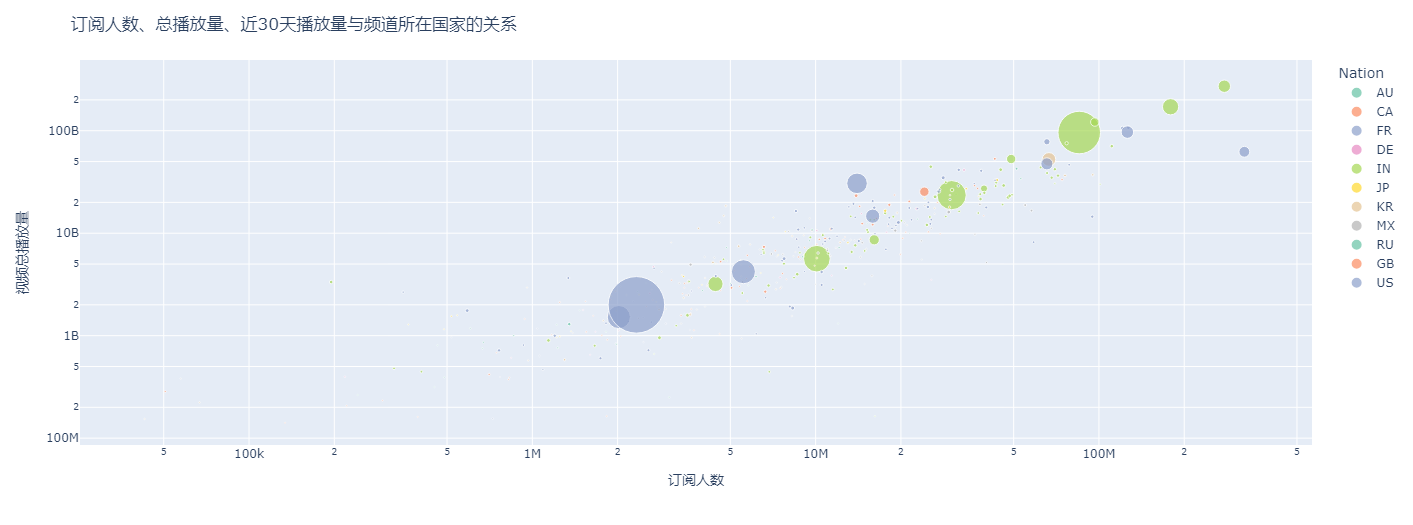
\includegraphics[width=0.7\textwidth]{pic/p2} %插入图片,[]中设置图片大小,{}中是图片文件名
%\caption{Main name 2} %最终文档中希望显示的图片标题
\label{Fig.p2} %用于文内引用的标签
\end{figure}

\begin{figure}[H] %H为当前位置,!htb为忽略美学标准,htbp为浮动图形
\centering %图片居中
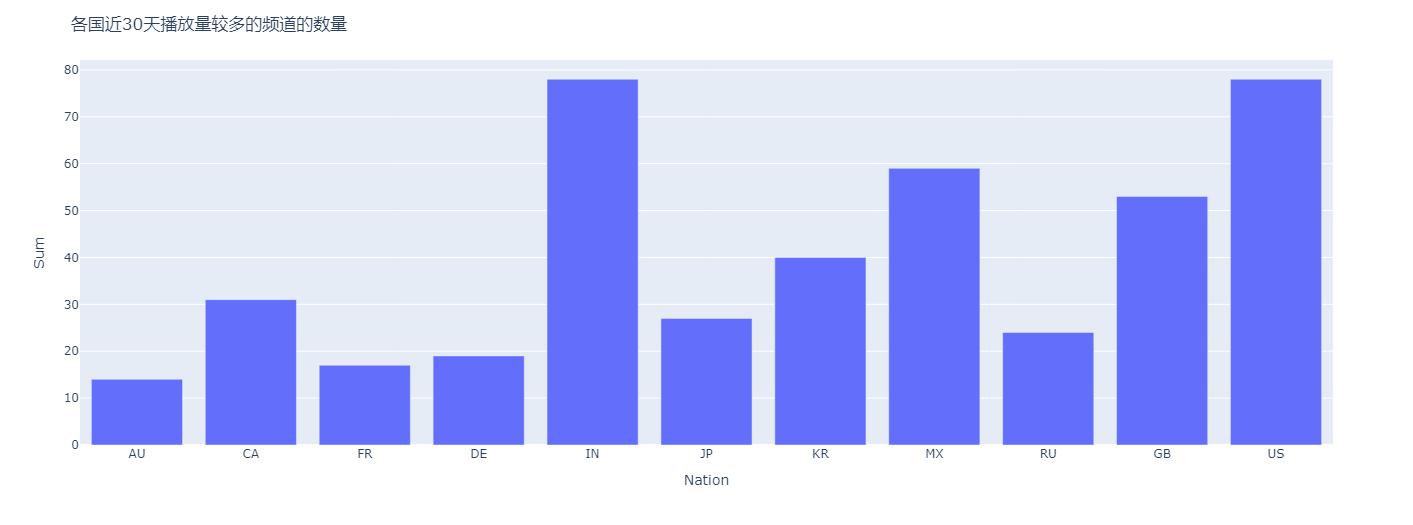
\includegraphics[width=0.7\textwidth]{pic/p3} %插入图片,[]中设置图片大小,{}中是图片文件名
%\caption{Main name 2} %最终文档中希望显示的图片标题
\label{Fig.p3} %用于文内引用的标签
\end{figure}

\begin{figure}[H] %H为当前位置,!htb为忽略美学标准,htbp为浮动图形
\centering %图片居中
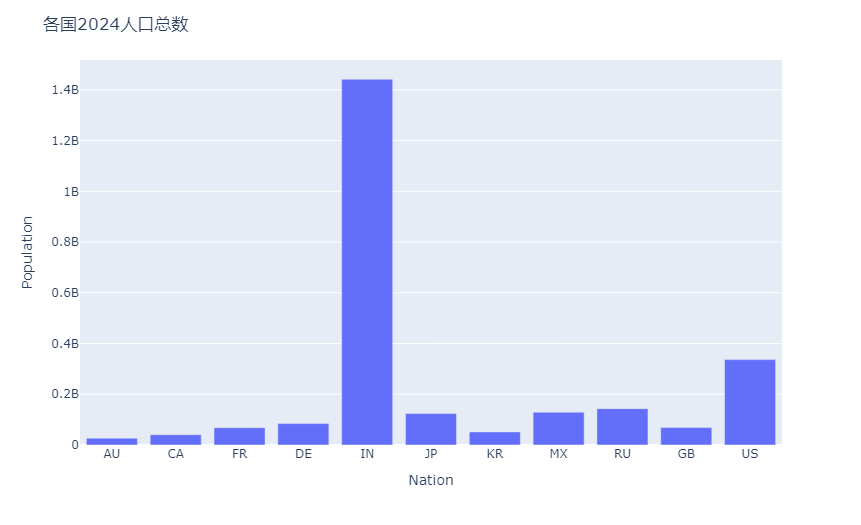
\includegraphics[width=0.7\textwidth]{pic/p4} %插入图片,[]中设置图片大小,{}中是图片文件名
%\caption{Main name 2} %最终文档中希望显示的图片标题
\label{Fig.p4} %用于文内引用的标签
\end{figure}

\begin{figure}[H] %H为当前位置,!htb为忽略美学标准,htbp为浮动图形
\centering %图片居中
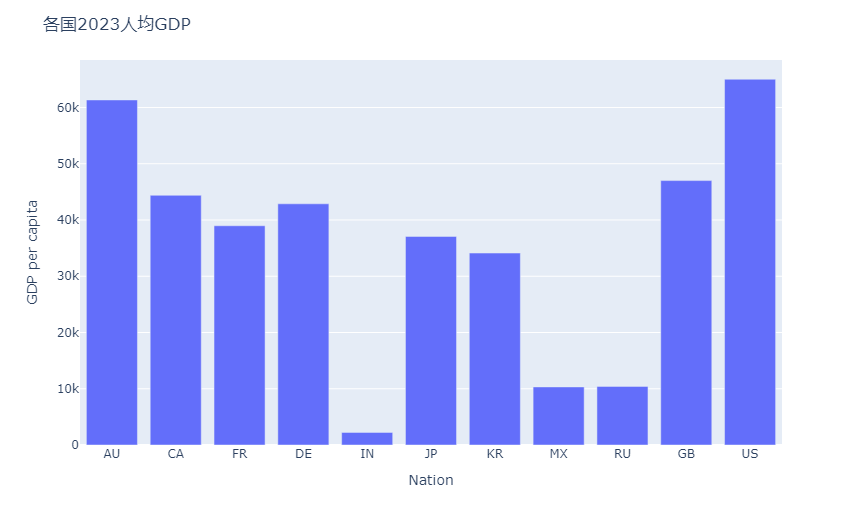
\includegraphics[width=0.7\textwidth]{pic/p5} %插入图片,[]中设置图片大小,{}中是图片文件名
%\caption{Main name 2} %最终文档中希望显示的图片标题
\label{Fig.p5} %用于文内引用的标签
\end{figure}

可以看出近30天播放量大于一亿的频道中,最火的频道集中于美国和印度,而且美国和印度的近30天播放量较大的频道的数目也是最多的。同时可看出,印度人口最多而人均GDP最低,美国人口数量第二而人均GDP最高,基于这个有趣的情况,可以进一步探索国家经济状况对于youtube频道注册的影响。

\section{任务分析}

我们暂定想要探索的任务为不同国家经济状况对youtube频道注册的影响;找找什么种类频道是人们感兴趣的。


\end{document}